\chapter{Lösungskonzept}
    \label{chapter:SolutionConcept}
    Dieses Kapitel erläutert ein Lösungskonzept für die in Kapitel \ref{chapter:ProblemAnalysis} beschriebene Problemstellung.
    Zentrale Elemente dieser Lösung sind ein System zur automatischen Klassifizierung der Inhalte von Webseiten
    und eine \gls{dsl} zu dessen Instrumentierung.
    Unter dem Namen \gls{wccs} wird im weiteren Verlauf dieser Arbeit
    Bezug auf diese Lösung genommen.

    \section{Vision}
    An dieser Stelle erfolgt zunächst ein sehr abstrakter Blick auf das System,
    um die Idee der Gesamtlösung zu vermitteln.
    Dazu wird die Vision des angestrebten Klassifizierungsprozesses beschrieben.

    Ein Anwender entwickelt ein Modell zur Klassifizierung einer oder mehrerer Webseiten,
    welches er mit Hilfe einer \gls{dsl} ausdrückt.
    Das Modell wird übersetzt und fungiert zur Instrumentierung des Klassifizierungssystems.
    Der Anwender startet anschließend ein geeignetes Werkzeug,
    welches alle relevanten Webseiten ermittelt und ihre Klassifizierung beauftragt.
    Das \gls{wccs} führt die Klassifizierung auf Basis des bereitgestellten Modells durch
    und persistiert das Ergebnis dauerhaft.
    Eine erste Überprüfung der Klassifikation und kleinere Korrekturen kann der Anwender anschließend auf der
    Webseite selbst vornehmen.
    Dazu dient eine Visualisierung über Webannotationen.
    Eine detailliertere Einsicht erhält er über eine spezielle Webanwendung.
    Nach der Klassifizierung steht Drittsystemen das Ergebnis über eine definierte Schnittstelle
    zur Verfügung.

    \section{Klassen, Features und Selektoren}
    \section{Eine domänenspezifische Sprache zur Spezifikation von Klassen}
    Das \gls{wccs} braucht für die Durchführung einer Klassifizierung
    eine Spezifikation, die die bekannten Klassen definiert.

    Hierzu bietet das \gls{wccs} eine domänenspezifsche Sprache:
    Die \gls{wccdl}.

    \subsection{Funktionen}
        Die Sprache greift die in Kapitel \ref{section:conceptClassesFeaturesSelectors}
        beschriebenen Konzepte auf.

        Zunächst erlaubt sie die Definition von benannten Klassen,
        wobei sie die Unterscheidung zwischen Seiten-, Inhalts und Referenzklassen
        erlaubt.
        Des Weiteren kann mit ihr ein Selektor für eine Klasse definiert werden,
        was im Falle von Seitenklassen zwingend erforderlich ist.

        Zu einer Klasse gehören wie beschrieben auch Features,
        die mit der \gls{wccdl} ebenfalls deklariert werden können.
        Neben dem Namen und der Klasse des Features, gehört dazu auch
        ein Selektor und ob es sich um ein mehrelementiges Feature handelt oder nicht.

        % TODO: Muss hier nochmal erwähnt werden, dass der Selektor optional ist?
        % TODO: Muss hier schon darauf hingewiesen werden, dass die Ermittlung ob Content oder ReferenceFeature anhand der Klasse passiert?

    \subsection{Generierungsergebnis}
        Anstatt in ein ausführbares Programme, wird Spezifikation in eine Konfigurationsdatei für
        das Klassifizierungssystem übersetzt.
        Die Sprache ist deklarativ, weshalb keine Anweisungen formuliert werden.
        Der übergeordnete Algorithmus ist deshalb immer gleich.
        Die Programme wärend deshalb zu großen Teilen identisch und unnötig komplex.
        Deshalb sinnvoller ihn auszulagern und Spezifikation lediglich in ein anderes Format zu übersetzen.
        % TODO: Kann das hier vielleicht lieber in die Einleitung. Dann ggf. ohne Begründung?

    \subsection{Vorteile}
        Die Verwendung einer DSL hat mehrere Vorteile.

        \paragraph{Erleichterte Konfiguration des Systems}
        Das technische Format der Konfigurationsdatei wird verborgen
        und die Spezifikation in einem lesbaren Format gespeichert.
        Das erlaubt die Formulierung der Klassendefinitionen prinzipiell auch
        Nicht-Programmierern.
        Selektoren müssen beispielsweise nicht für das technische Format manuell escaped werden,
        was ihre Formulierung erleichtert.

        \paragraph{Fehlervermeidung}
        Dadurch, dass wir mit einer Sprache arbeiten, die in ein Artefakt generiert wird,
        können Fehler besser abgefangen werden.
        Z. B. durch syntaktische Korrektheit oder semantische Validitätsprüfungen.
        Ein Beispiel sind die zur Verfügung stehenden Selektoren und ihre semantisch korrekte Verwendung.
        Genauso kann sichergestellt werden, dass für jedes Feature ein Selektor ableitbar ist.

        \paragraph{Leichtere Wiederverwendbarkeit}
        Durch die logische und physische Aufteilung können Klassendefinitionen leichter
        wiederverwendet oder übertragen werden, als dies bei der direkten Verwendung eines
        technischen Formates wäre.

        \paragraph{Unabhängigkeit vom konkreten Klassifizierungssystem}
        Die Sprache ist unabhängig von der konkreten Implementierung des Klassifizierungssystem.
        Es ist deshalb möglich für verschiedene Implementierungen verschiedene Dateien zu generieren.
    \subsection{Klassifizierung einer Webseite}
    \label{section:solutionDetailsClassificationServiceClassification}
    Dieser Abschnitt geht detaillierter auf die Klassifizierung einer Webseite ein
    und beschreibt einige Aspekte der Umsetzung.

    \paragraph{Ablauf}
    Die Klassifizierung folgt einem Algorithmus,
    der rekursiv die Features einer Seitenklasse abarbeitet und nach Entsprechungen
    auf einer Webseite sucht.
    Er ist in Listing \ref{listing:classificationAlg} skizziert.

    \lstinputlisting[
        label=listing:classificationAlg,
        caption=Der Klassifizierungsalgorithmus,
        style=pseudo
    ]{../resources/classification.code}

    Die Klassifizierung nutzt die HTML-Repräsentation einer
    Webseite\footnote{vgl. Kapitel \ref{section:conceptClassificationDataSource}},
    weshalb diese zunächst über ihre \gls{url} bezogen und geparst wird,
    wodurch ein \gls{dom} entsteht.
    Mit diesem können Inhalt, Struktur und Aussehen der Webseite
    dynamisch abgefragt werden \cite{w3c:dom}.
    Anschließend wird die Klasse der Seite ermittelt,
    indem bis zur ersten Übereinstimmung der Selektor jeder bekannten
    Seitenklasse auf die Webseite angewandt wird.
    Danach beginnt die Ermittlung der Features der ermittelten Seitenklasse.
    Dazu ruft der Algorithmus die Funktion \texttt{classify} auf,
    die eine Liste der zu suchenden Features und ein HTML-Element erwartet.
    Letzteres bestimmt den Kontext, in dem die Suche stattfindet\footnote{vgl. Kapitel \ref{section:conceptSupportedSelectors}}.
    Im ersten Schritt ist dies das DOM-Objekt \texttt{document},
    welches das gesamte HTML-Dokument widerspiegelt \cite[Kapitel 1.4]{w3c:dom}.
    Für jedes Feature durchläuft die Funktion die gleichen Schritte.
    Zunächst sucht sie innerhalb des Kontextobjektes nach allen Elementen,
    die dem Selektor des aktuellen Features entsprechen.
    Falls das Feature ein {\scalarFeature} ist, behält sie allerdings nur den ersten Treffer.
    Die Klassifikation der Elemente wird anschließend gespeichert.
    Dabei wird sowohl der textuelle Inhalt bzw. die \gls{url}
    der referenzierten {\resource} als auch ein eindeutiger Selektor eines Elementes ermittelt
    und gespeichert\footnote{vgl. Kapitel \ref{section:conceptPageDataModel}}.
    Handelt es sich um ein {\collectionFeature}, ruft sich \texttt{classify} anschließend rekursiv für jedes klassifizierte Element auf.
    In jedem Aufruf verwendet sie als Parameter die {\childFeature}s der Klasse sowie das klassifizierte HTML-Element.

    \paragraph{Browserautomatisierung}
    Die Herausforderung bei der Implementierung dieses Algorithmus
    ist die Auswertung der Selektoren und das dazu notwendige Parsen des \gls{html}-Dokumentes.
    Das \gls{wccs} setzt zur Bewältigung dieser Aufgabe auf die Automatisierung eines Webbrowsers.
    Konkret verwendet es die Bibliothek
    Puppeteer\footnote{\url{https://github.com/GoogleChrome/puppeteer}},
    mit deren Hilfe sich der Browser Google Chrome ohne die Anzeige einer graphischen Oberfläche starten
    und anschließend programmatisch steuern lässt.
    Der wichtigste Vorteil der Nutzung eines echten Browsers ist seine ausgereifte und umfangreiche Implementierung
    als Parser von \gls{html}, CSS und XPath.
    Des Weiteren führt der Webbrowser das auf der Seite enthaltene JavaScript aus,
    was für die Klassifizierung von Bedeutung sein kann.

    \paragraph{Selektoren}
    Dank Puppeteer kann zur Umsetzung der Selektoren auf standardisierte Schnittstellen
    zurückgegriffen werden, die die benötigten Informationen liefern.
    Der {\cssSelector} kann die Methode \texttt{querySelectorAll} nutzen,
    die sowohl auf \texttt{document} als auch auf beliebigen \gls{html}-Elementen verfügbar ist
    \cite[Kapitel 6.1]{w3c:selectorsAPI}.
    Diese Methode wertet CSS-Ausdrücke auf der Webseite aus und gibt alle gefundenen Elemente zurück,
    die Kinder des Elementes sind, auf dem sie aufgerufen
    wurde\footnote{vgl. Kapitel \ref{section:conceptSupportedSelectors}}.

    Der {\xpathSelector} wird hingegen über die Methode \texttt{evaluate} des Objektes \texttt{document} realisiert
    \cite[Kapitel 1.4]{w3c:domXPath}.
    Diese Methode erwartet neben dem XPath-Ausdruck auch ein Kontextobjekt,
    sodass auch hier der beschriebene Algorithmus leicht umgesetzt werden kann.
    Das Ergebnis dieser Methode kann abhängig vom XPath-Ausdruck eine Liste von HTML-Elementen, eine Zeichenkette,
    ein boolescher Wert oder eine Zahl sein
    \cite[Kapitel 1.4]{w3c:domXPath}.
    Die beiden zuletzt genannten werden vom \gls{wccs} nicht unterstützt und als keine Übereinstimmung mit dem Selektor gewertet.
    Bei HTML-Elementen wird der Algorithmus wie beschrieben weiter durchlaufen.
    Im Falle von Zeichenketten wird die Rekursion allerdings unterbrochen, da kein neues Element vorhanden ist,
    welches den Suchraum weiter einschränken könnte.
    Abhängig von der Art des Features wird die Zeichenkette als textueller Inhalt
    oder als \gls{url} einer referenzierten {\resource} interpretiert.
    Durch die Verwendung von \texttt{document.evaluate} ist ein {\xpathSelector}
    auf die Möglichkeiten von XPath 1.0 eingeschränkt \cite{w3c:domXPath}.

    Der {\urlSelector} ist für Webseiten und Features unterschiedlich implementiert.
    Im Falle von Seiten wird der reguläre Ausdruck auf ihre \glspl{url} angewandt.
    Eine Übereinstimmung wird als Erfüllung des Selektors gewertet.
    Für Features werden zunächst alle Elemente innerhalb des Kontextobjektes gesucht, die {\resources} referenzieren.
    Das sind diejenigen Elemente, die eines der Attribute \texttt{href}, \texttt{src} oder \texttt{srcset} besitzen
    \cite[Kapitel 4.7, 4.8]{w3c:html5}.
    Um diese Elmente zu finden, wird der {\cssSelector} \texttt{[href], [src], [srcset]} auf dem Kontextobjekt ausgeführt.
    Anschließend wird für jeden Treffer der Wert des gefundenen Attributes ausgelesen
    und der reguläre Ausdruck des {\urlSelector}s auf ihm angewandt.
    Bei einer Übereinstimmung wird das Element in die Ergebnismenge aufgenommen.

    Aus diesen Beschreibungen folgt, dass Selektoren selbst keine Unterscheidung bez.
    der Kardinalität eines Features machen.
    Stattdessen liefern sie immer alle Treffer und überlassen dem Aufrufer die Aufgabe zu entscheiden,
    welche Elemente er verwendet.
    Das wird auch in Listing \ref{listing:classificationAlg} deutlich.

    \paragraph{Textueller Inhalt und Referenzziel eines Features}
    Ein {\contentFeature} speichert seinen textuellen Inhalt und ein {\referenceFeature}
    die \gls{url} seines Zieles\footnote{vgl. Kapitel \ref{section:conceptPageDataModel}}.
    Bei {\contentFeature}s gilt allerdings die Einschränkung, dass nur solche ihren textuellen Inhalt speichern,
    bei denen sich kein {\contentFeature} unter den {\childFeature}s befindet.
    Der Grund ist, dass durch solche {\childFeature}s der Text spezieller klassifiziert und
    feingranularer gespeichert werden kann.
    Inhalt bzw. Ziel müssen während der Klassifizierung ermittelt werden.
    Für {\contentFeature}s nutzt das \gls{wccs} die Eigenschaft \texttt{innerText} des klassifizierten HTML-Elementes.
    Anders als \texttt{textContent} enthält diese Eigenschaft nur den gerenderten Text,
    wodurch \texttt{style}- und \texttt{script}-Elemente sowie Kommentare und Zeilenumbrüche im Quelltext
    ausgeschlossen werden
    \cite[Kapitel 3.2.7]{whatwg:html}.
    Für den Anwendungsfall des \gls{wccs} ist \texttt{innerText} deshalb besser geeignet als \texttt{textContent}.
    Die \gls{url} einer {\resource} bezieht das \gls{wccs} aus dem Attribut
    \texttt{href}, \texttt{src} oder \texttt{srcset} des klassifizierten HTML-Elementes.

    \paragraph{Bestimmung eines eindeutigen Selektors}
    Eine vollständige Klassifikation enthält für jedes Feature auch einen eindeutigen
    Selektor des klassifizierten HTML-Elementes\footnote{vgl. Kapitel \ref{section:conceptPageDataModel}}.
    Da diese Information von Annotator benötigt wird,
    um Annotationen zu erzeugen,
    orientiert sich das \gls{wccs} für den Aufbau und das Format eines Selektors
    an dieser Bibliothek.
    Ein Selektor besteht demnach aus vier Elementen
    \cite[Kapitel "`Annotation format"']{annotator:documentation}:
    Zwei XPath-Ausdrücken, die ein Start- und ein Endelement identifizieren
    sowie zwei numerischen Angaben, die Positionen in diesen Elementen festlegen.
    Dadurch kann Annotator eine Annotation an einer beliebigen Stelle eines Elementes beginnen
    und innerhalb eines anderen Elementes beenden.
    Im Falle des \glspl{wccs} sind Start- und Endelement immer identisch,
    da mit den Selektoren des {\classificationModel}s genau ein Element
    oder Text innerhalb eines Elementes erfasst wird.
    Die Versatzangaben bestimmen dabei, welcher Bereich dieses Elementes klassifiziert wurde.
    Mit der Selection API des \glspl{w3c} \cite{w3c:selectionAPI} lassen sich diese Angaben bestimmen,
    was dem \gls{wccs} prinzipiell eine einfache und standardisierte Methode eröffnet.
    Annotator folgt allerdings einem eigenen Algorithmus,
    der nach eigenen Versuchen andere Resultate liefert als die Selection API.
    Selektoren, die mit der Selection API bestimmt wurden,
    setzt Annotator deshalb nicht den Erwartungen entsprechend in Annotationen um.
    Würde das \gls{wccs} bei der Bestimmung eines eindeutigen Selektors Annotators
    Algorithmus folgen, müssten Drittsysteme diesen kennen,
    um die Angaben korrekt interpretieren zu können.
    Das \gls{wccs} verwendet deshalb einen Mittelweg,
    der sowohl gute Ergebnisse in Annotator liefert,
    als auch leicht durch Drittsysteme nachvollzogen werden kann.
    Die XPath-Ausdrücke sind absolute Angaben, die immer dasselbe Element erfassen und aufgrund ihrer Standardisierung
    für jedes Drittsystem eindeutig zu interpretieren sind.
    Das \gls{wccs} folgt bei der Berechnung dieser Ausdrücke Annotators Vorgehen,
    um eine größtmögliche Kompatibilität zu erzielen.
    Ausgehend von einem Element wird der Vaterkette bis zur Wurzel des \gls{html}-Dokumentes
    gefolgt und dabei die Namen und Positionen der besuchten Elemente gesammelt.
    Aus diesen Informationen lässt sich ein eindeutiger XPath-Ausdruck erzeugen.
    Wurde durch den Selektor des {\classificationModel}s ein vollständiges Element klassifiziert,
    ist der Versatz im Startelement 0, im Endelement die Länge der Eigenschaft \texttt{innerText}.
    Das führt bei Annotator meist zum richtigen Ergebnis.
    Falls durch einen {\xpathSelector} eine Zeichenkette in einem Element erfasst wurde,
    berechnen sich Start- und Endversatz wie folgt, wobei die Variable \texttt{text} den klassifizierten Text bezeichnet:

    \begin{lstlisting}
startOffset = node.innerText.indexOf(text)
endOffset = startOffset + text.length
    \end{lstlisting}
    
    Diese Berechnung ist leicht nachzuvollziehen,
    führt bei Annotator in manchen Fällen aber zu leicht verschobenen
    Annotationen\footnote{vgl. Kapitel \ref{section:findingsTeachersAbnormalitiesBabw}}.

    \paragraph{Parallelisierung}
    Mit dem beschriebenen Verfahren können prinzipiell beliebig viele Webseiten parallel klassifiziert werden.
    Bei sehr vielen gleichzeitigen Anfragen dürfen aber nicht alle Seiten
    gleichzeitig über Puppeteer im Browser geöffnet werden.
    Die Anzahl der dadurch erzeugten Prozesse kann zum Einfrieren des Systems führen.
    Aus diesem Grund begrenzt der {\classificationService} die Anzahl der gleichzeitig klassifizierten Webseiten
    und verwaltet eine Warteschlange seiner Aufträge.
    Es ist außerdem möglich, die Klassifizierung einer einzelnen Webseite zu parallelisieren.
    Zwischen Features mit demselben direkten {\parentFeature} besteht nämlich keine Abhängigkeit,
    sodass sie nebenläufig abgearbeitet werden können.

    \section{Visualisierung, Nachbesserung und Prüfung der Klassifikation}
    \label{section:conceptVisualization}
    Es ist möglich, dass eine Klassifizierung ein teilweise unerwartetes Ergebnis liefert,
    weil zum Beispiel Selektoren im Klassifizierungsmodell unzutreffend sind.
    Das \gls{wccs} bietet deshalb Möglichkeiten,
    um eine Klassifikation zu visualisieren und zu prüfen.

    \subsection{Webannotationen}
        \label{section:conceptWebAnnotations}
        % TODO: LINK AUF W3C Standard (https://www.w3.org/annotation/), aber den verwenden wir gar nicht?
        Die Visualisierung der Klassifikation geschieht über Webannotationen,
        wodurch die klassifizierten Inhalte und Referenzen direkt in der Webseite hervorgehoben werden.
        Der Inhalt der Annotation ist die Klasse des annotierten Elementes.
        Beispiele annotierter Webseiten zeigen die Abbildungen
        \ref{image:findingTeachersAnnotationsOverview},
        \ref{image:annotatorPluginViewer} und \ref{image:annotatorPluginEditor}.

        Eine Annotation spiegelt ein {\referenceFeature} oder ein
        {\contentFeature} ohne untergeordnete {\contentFeature}s wieder.
        Wäre jedes {\contentFeature} durch eine Annotation hervorgehoben,
        überlagerten sich die Annotationen unter Umständen mehrfach,
        wodurch sich die Übersichtlichkeit
        und damit der Nutzen der Annotationen deutlich verschlechtern würde.
        Durch Annotationen wird somit die Klassifikation auf der feingranularsten Ebene visualisiert.
        Eine Überlagerung ist aber weiterhin möglich,
        wenn ein {\contentFeature} ausschließlich untergeordnete {\referenceFeature}s besitzt,
        weil dann die Annotation des textuellen Inhalts teilweise durch die
        der Referenzen überlagert wird.
        Eine Unterscheidung ist trotzdem möglich\footnote{vgl. Kapitel \ref{section:solutionDetailsAnnotatorPlugin}}.
        
        Neben der Visualisierung dienen Annotationen auch der Korrektur der Klassifikation.
        Bearbeitet ein Nutzer nämlich eine Annotation,
        ändert er damit die Klasse des Features.

        Diese Funktion realisiert das \gls{wccs} über eine Erweiterung der JavaScript-Bibliothek
        Annotator\footnote{vgl. \ref{section:solutionDetailsAnnotatorPlugin}}.
    
    \subsection{Webanwendung}
        Über Webannotationen ist es nicht möglich anschaulich alle Details einer Klassifikation darzustellen
        oder einen Überblick über alle klassifizierten Seiten zu geben.
        Zu diesem Zweck stellt das \gls{wccs} deshalb auch eine Webanwendung bereit,
        die diese Lücken schließt.
        Die Oberflächen dieser Anwendung sind in Kapitel \ref{section:solutionDetailsWebAppFunctions}
        enthalten.

    \section{Bereitstellung der Klassifikation}
    Drittsysteme sollen die Möglichkeit haben,
    die Klassifikation für eine bestimmte Seite beim \gls{wccs} anzufragen.
    Dazu bietet es zwei Alternativen:

    \begin{enumerate}
        \item Einen RESTful Webservice
        \item Direkter Zugriff auf die Datenbank
    \end{enumerate}

    Eine Klassifikation kann beim Webservice anhand der \gls{url} der Webseite angefragt werden,
    da diese ein eindeutiges Merkmal darstellt.
    Die Antwort folgt dem beschriebene Datenmodell einer
    Klassifikation\footnote{vgl. \ref{section:conceptPageDataModel}}.

    Durch den direkten Zugriff auf die Datenbank können
    beliebige individuelle Sichten auf die Daten oder Abfragen realisiert werden.

    \section{Werkzeug zum Auffinden aller zu klassifizierenden Seiten}
    \section{Architektur}
    \label{section:Architecture}
    Das \gls{wccs} verwendet eine Microservices-Architektur.
    Dieses Muster wird in diesem Kapitel zuerst vorgestellt.
    Anschließend erläutert es die konkrete Architektur des Systems.

    \subsection{Microservices Architekturen}
        \label{section:conceptMicroServices}
        \paragraph{Prinzipien}
            ZUSTANDSLOSIGKEIT WIRD IN ANNOTATION SERVICE gebraucht!
        \paragraph{Vorteile}
        \paragraph{Herausforderungen}

    \subsection{Architektur}
        % TODO Sollte WCCS component lieber WCCS service sein? Was mit DSL oder Crawler? Was wären das dann?
        Architektur wird in zwei Schritten vorgestellt.
        Zunächst ein Blick in den internen Aufbau und anschließend auf die Zusammenhänge mit der Außenwelt.
        
        Abbildung \ref{image:wccsInternalArchitecture} legt den Fokus auf die
        internen Abläufe und Komponenten.

        \begin{figure}
            \centering
            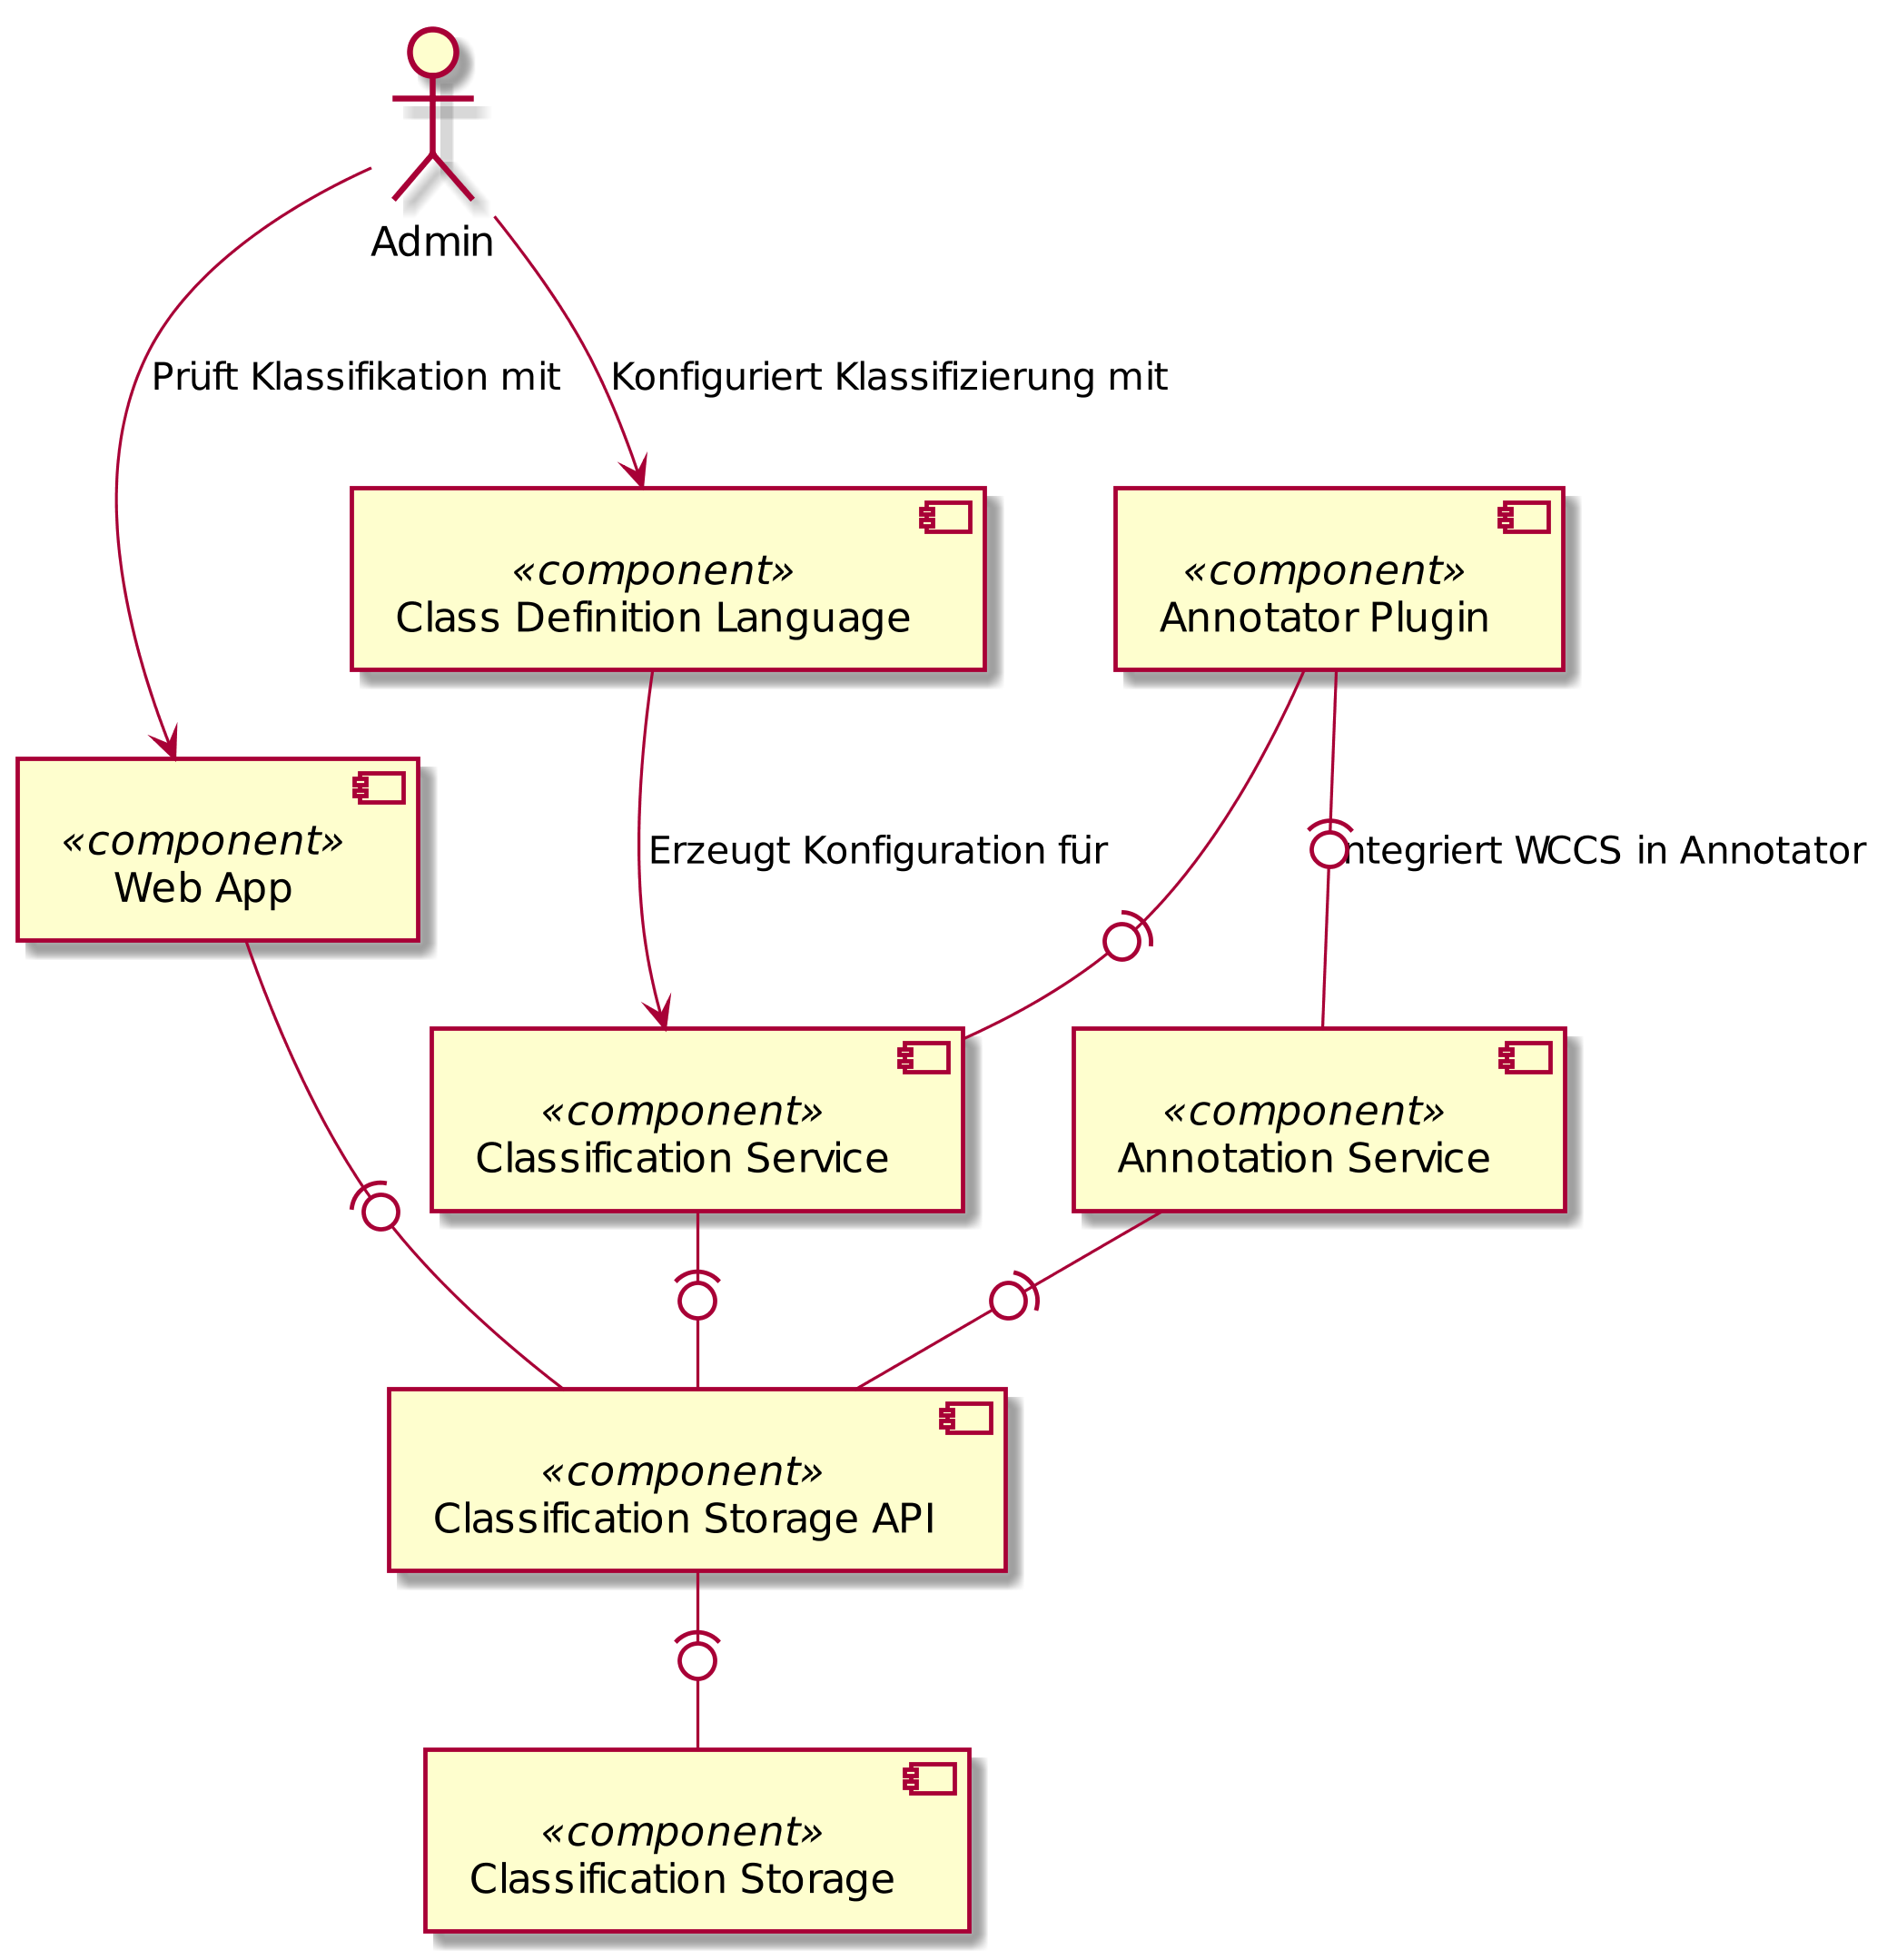
\includegraphics[width=0.7\textwidth]{../resources/architecture/wccs_internal_architecture.png}
            \caption{Interne Architkektur von WCCS}
            \label{image:wccsInternalArchitecture}
        \end{figure}

        Das \gls{wccs} besteht aus fünf Services im Sinne einer Micro-Services-Architektur.
        Dem Classification Storage, der Classification Storage API, dem Classification Service, dem
        Annotation Service und der Web App.

        Der Service Classification Storage stellt die Persistenz bereit und speichert
        Klassifikationen in einer Datenbank.
        Seine Schnittstelle entspricht der der verwendeten Datenbank und ist deshalb
        technisch orientiert.
        Mehr dazu in Kapitel \ref{section:solutionDetailsPersistence}.

        Die Classification Storage bietet eine fachliche Schnittstelle für die Datenhaltung.
        Er übersetzt deshalb fachliche Anfragen in Anfragen in der Sprache der Datenbank.
        Dementsprechend ist die konkrete Implementierung dieses Services abhängig vom Classification Storage.
        Die Schnittstelle der API - eine REST-Schnittstell - ist allerdings fachlich und deshalb
        unabhängig. Mehr zu diesem Service steht in  Kapitel \ref{section:solutionDetailsStorageAPI}.

        Der Classification Service führt die eigentliche Klassifizierung durch
        und speichert das Ergebnis über die Classification Storage API.
        Der Service kann ebenfalls über eine REST-Schnittstelle angesprochen werden.
        Mehr zum Service steht in Kapitel \ref{section:solutionDetailsClassificationService}.

        Der Annotation Service transformiert eine Klassifikation,
        die er über den Classification Storage bezieht,
        in eine Menge von Annotationen.
        Neben der Abfrage von Annotationen bietet seine Schnittstelle auch
        die Möglichkeit solche zu aktualisieren.
        Das technische Format orientiert sich an dem der Annotation Library.
        Mehr steht in Kapitel \ref{section:solutionDetailsAnnotationService}.

        Der verbliebene Service - die Web App - ist im Kern ein Web-Server,
        der die Web Anwendung bereitstellt,
        mit der der Nutzer die Klassifikation prüfen kann.
        Diese bezieht die Anwendung über die Classification Storage API ab.

        Neben diesen Services besitzt das System weitere Komponenten:
        Die Web Content Class Definition Language und das Plugin für die
        Annotation Library.
        Die Sprache nutzt der Admin, um eine Konfigurationsdatei für den
        Classification Service zu erstellen.
        Mehr zur Sprache in Kapitel \ref{section:solutionDetailsDSL}.
        Das Annotator Plugin stellt eine Integration des \gls{wccs} in
        Annotator dar.
        Es bezieht die Annotationen einer Seite über den Annotation Service
        und Informationen über bekannte Klassen vom Classification Service.
        Beides ist notwendig, um einem Anwender die Klassifikation zu visualisieren
        und modifizierbar zu machen.
        Details in Kapitel \ref{section:solutionDetailsAnnotatorPlugin}.

        Die bisherige Betrachtung beantwortet noch nicht die Fragen,
        von wem der Classification Service angesprochen wird und wer das Annotator Plugin einbindet.
        Genauso ist noch offen, welche weiteren Beziehungen zur Umgebung bestehen.

        Das stellt Abbildung \ref{image:wccsExternalArchitecture} dar
        und enthält neben einigen Komponenten des \gls{wccs} vor allem auch
        externe Komponenten.

        \begin{figure}
            \centering
            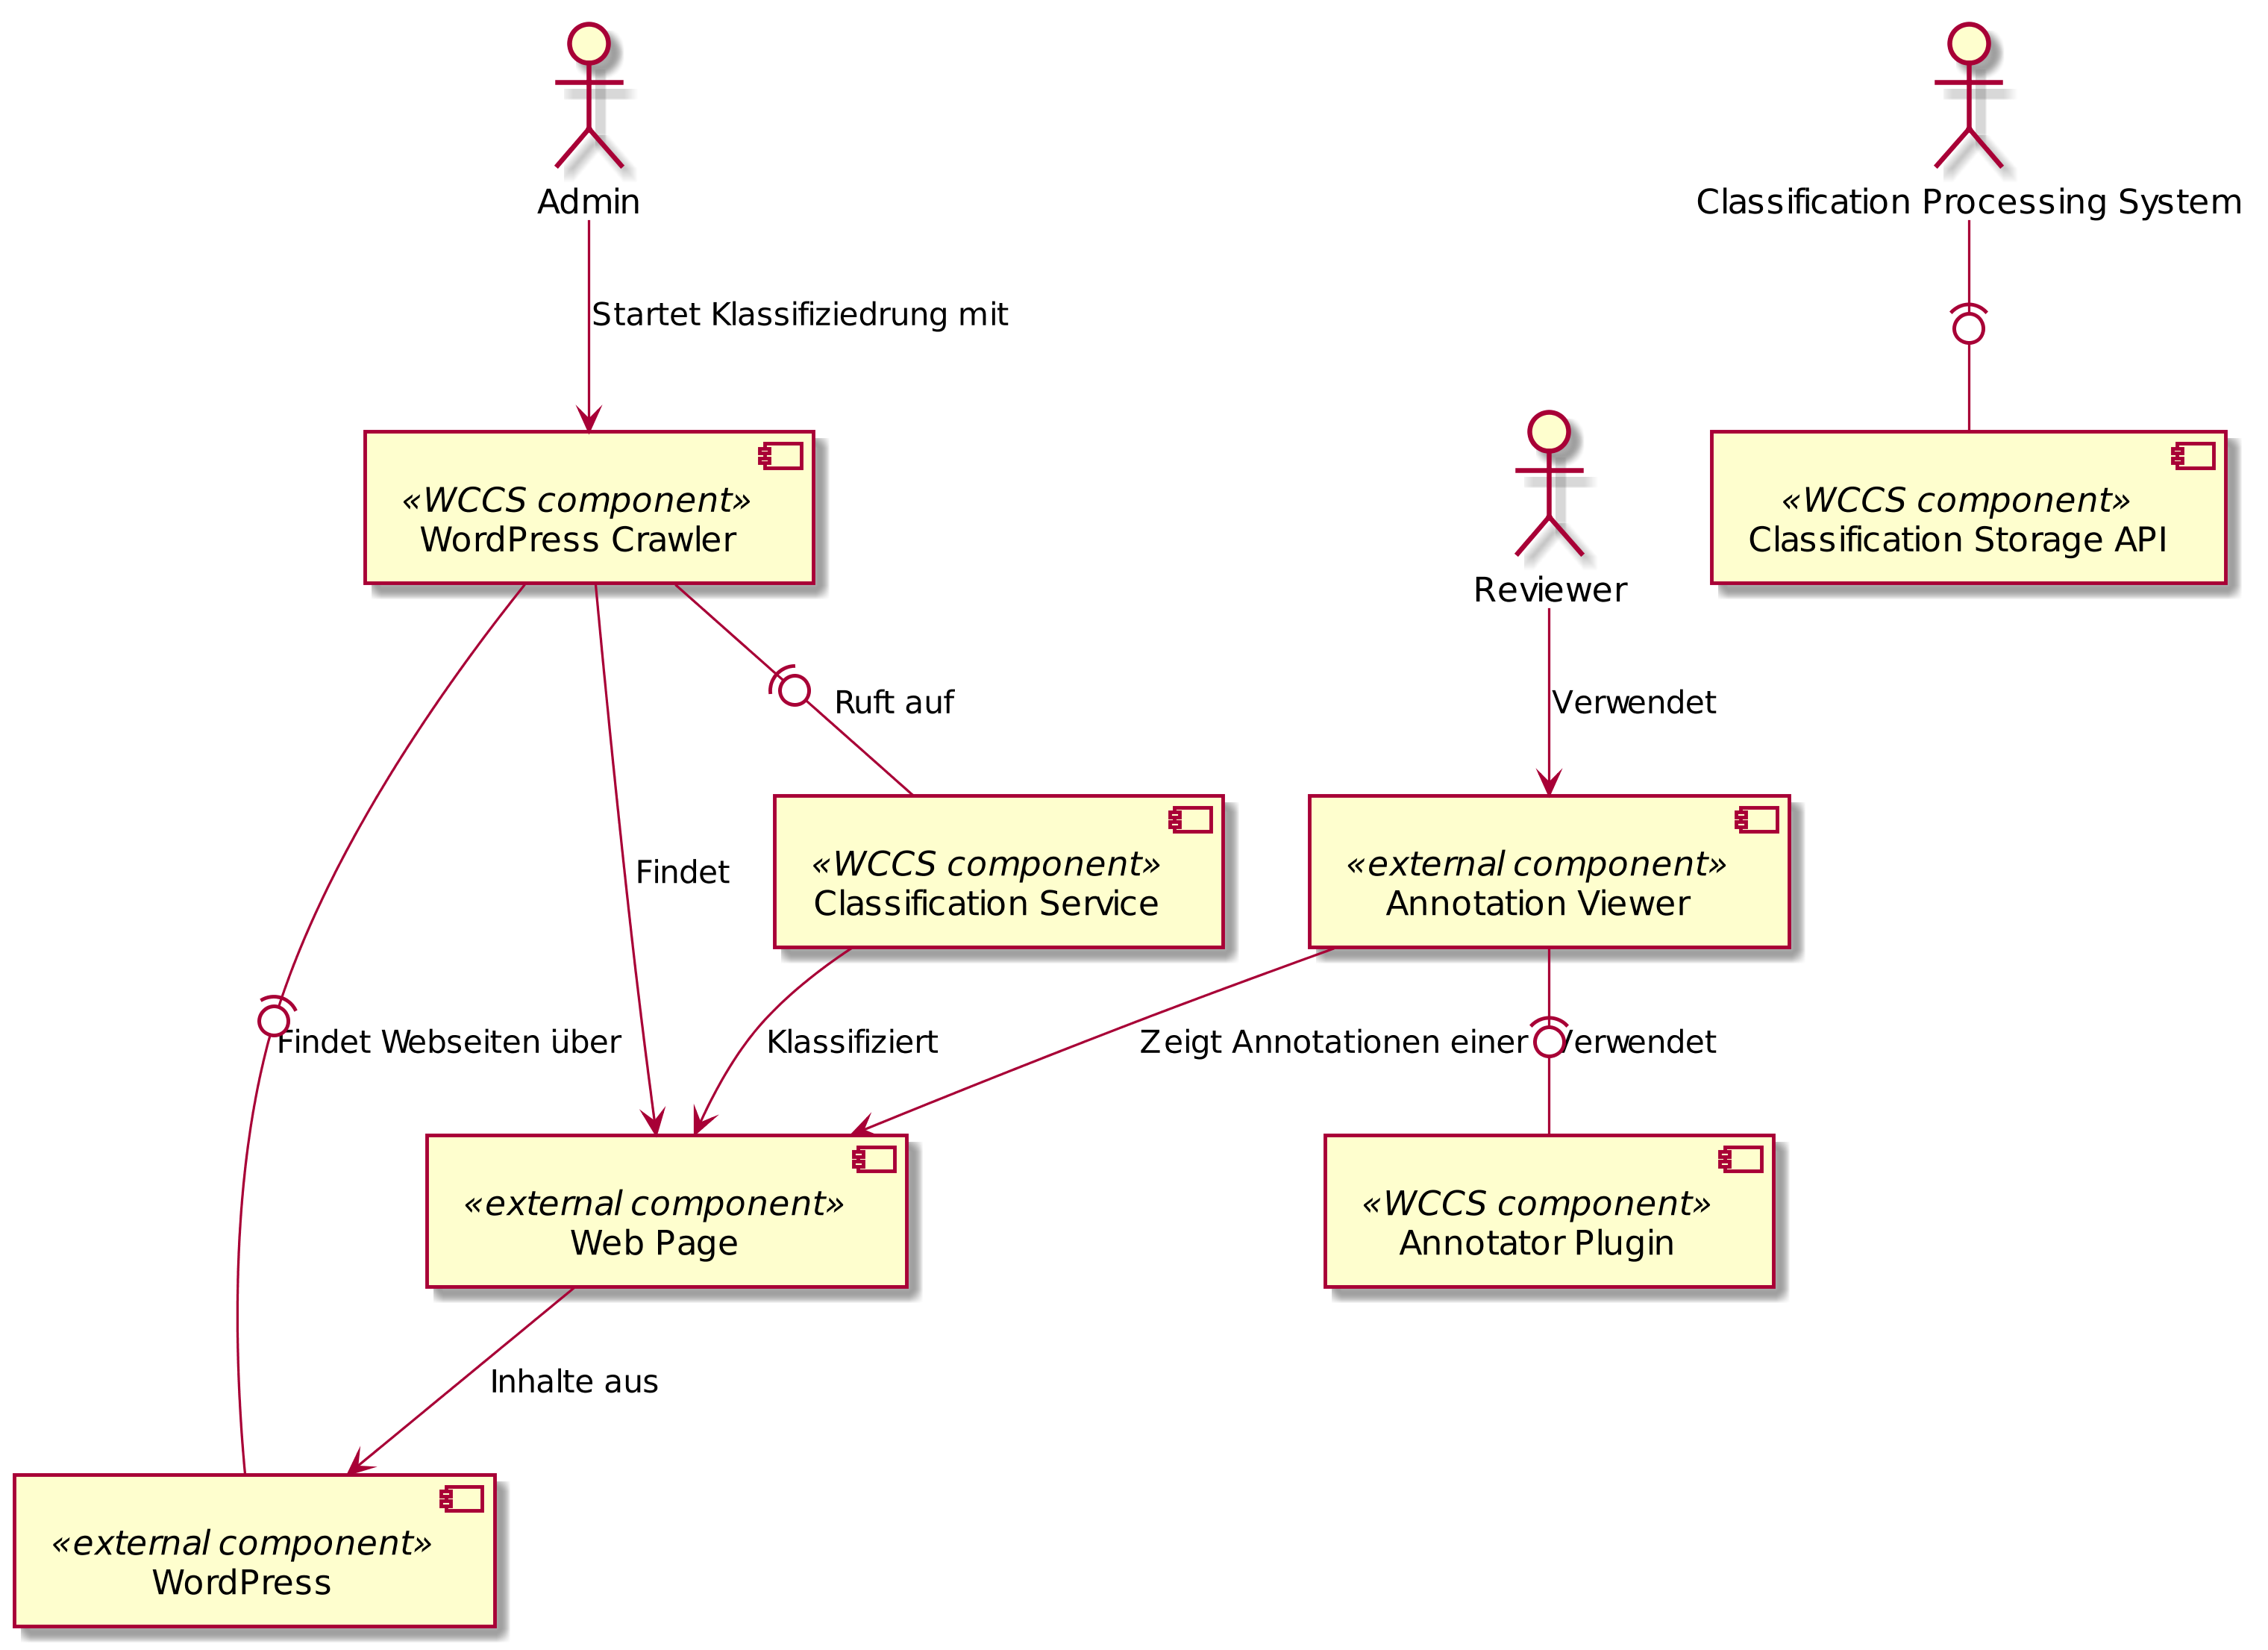
\includegraphics[width=\textwidth]{../resources/architecture/external_architecture.png}
            \caption{Externe Architkektur von WCCS}
            \label{image:wccsExternalArchitecture}
        \end{figure}

        Eine zentrale externe Komponente ist die Webseite,
        die Inhalte aus einem \gls{cms} - im konkreten Fall {\wordpress} -
        darstellt und vom Classification Service klassifiziert wird.
        Dazu startet der Admin den WordPress Crawler, der ebenfalls ein Teil des \gls{wccs} ist.
        Diese Komponente findet Webseiten über {\wordpress} und beauftragt den
        Classification Service diese zu klassifizieren.
        Obwohl Crawler Teil des \gls{wccs} ist, steht sie etwas außerhalb,
        da sie nur mit {\wordpress} funktioniert. Für andere Systeme muss ein anderes Tool
        entwickelt werden. Deshalb ist sie nicht so allgemeingültig.
        Konzeptionell gibt es aber immer so eine Komponente.
        Mehr in Kapitel \ref{section:solutionDetailsCrawler}.

        Nach der Klassifizierung kann eine externe Komponente das Annotator Plugin
        einbinden und damit die Annotationen visualisieren.
        Diese Komponente heißt deshalb Annotation Viewer und wird von einem Redakteur
        verwendet.

        Letzendlich können beliebige Drittsysteme die Classification Storage API
        nutzen, um Klassifikationen abzufragen und weiterzuverarbeiten.
